% !TeX root = main.tex

\section{Introduction}

\subsection{Présentation de la structure d'accueil}

Le cabinet GEO-SIAPP est une société de géomètres-experts dont le siège est implanté à Aubenas, en Ardèche, depuis 1992. Ce territoire est particulièrement vaste et à forte dominante rurale, ce qui nécessite une proximité constante avec le terrain et la clientèle. Pour couvrir ce territoire, GEO-SIAPP s'est développé autour de quatre agences, comme le montre la figure~\ref{fig:carte_agences} : Aubenas, Pierrelatte, Vallon-Pont-d'Arc et Guilherand-Granges.

Au fil de sa croissance, GEO-SIAPP a acquis plusieurs études de géomètres-experts locales. Ces acquisitions ont intégré de nouveaux collaborateurs mais aussi les archives de ces structures, dont certaines datent de plusieurs décennies. Le cabinet conserve ainsi une grande quantité de documents anciens, et pour la plupart manuscrits.

L'entreprise intervient sur l'ensemble des missions de la profession : le foncier (bornage, division parcellaire, mise en copropriété), l'urbanisme réglementaire, l'ingénierie VRD (maîtrise d'œuvre pour la voirie et les réseaux divers) ainsi que la topographie (photogrammétrie, relevés par drone,bathymétrie et scanner laser 3D).

\begin{figure}[H]
  \centering
  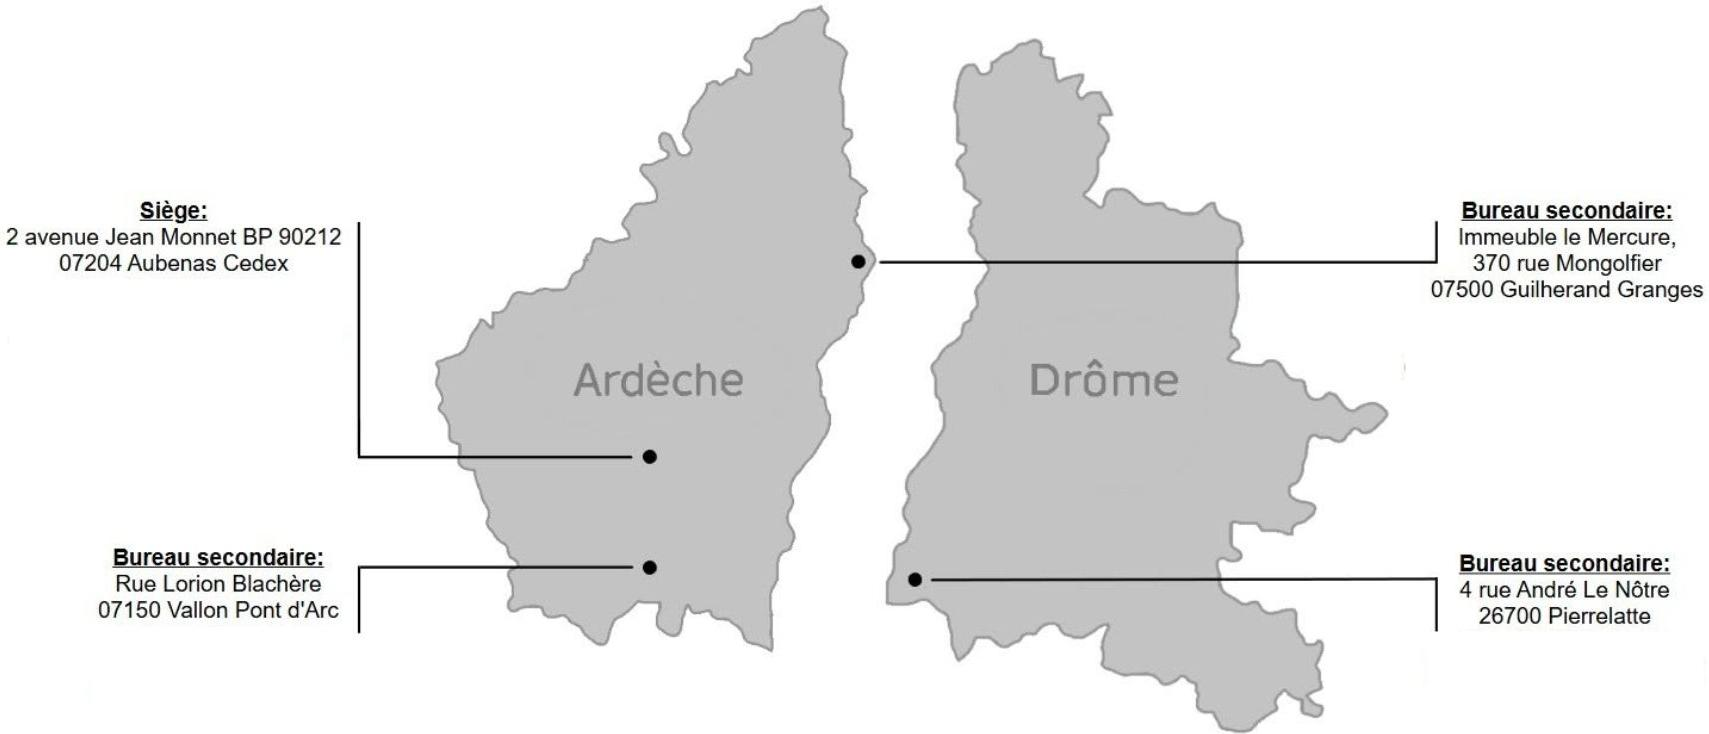
\includegraphics[width=\textwidth]{img/bureau_cropped.jpg}
  \caption{Implantation territoriale de GEO-SIAPP. La présence de quatre agences permet de répondre aux contraintes géographiques du département et explique la décentralisation des fonds d'archives. (Source~: \url{https://www.geo-siapp.com/index.php})}
  \label{fig:carte_agences}
\end{figure}

Ce projet de fin d'études s'est déroulé au sein du cabinet sur une période de six mois, de février à juillet 2026. La mission confiée consistait à concevoir et développer de bout en bout un outil informatique de traitement automatisé de ces archives, en vue de leur versement sur Géofoncier, le portail informatique national de la profession.

\subsection{Le cadre réglementaire et professionnel}

La profession de géomètre-expert est strictement réglementée, tout comme la gestion de la donnée foncière qu'elle produit et dont elle dispose du monopole légal en matière de fixation des limites de propriétés (loi du 7 mai 1946 \citep{loi_1946_geometre}). Le décret n°96-478 du 31 mai 1996 précise les obligations de la profession : seul le géomètre-expert est habilité à dresser les documents topographiques servant à la définition des droits fonciers \citep{decret_1996_geometre}. Par conséquent, chaque acte signé par le professionnel possède une valeur juridique opposable aux tiers et peut être produit en justice à tout instant.

En vertu de l'article 55 de ce même décret, le géomètre-expert a l'obligation de conserver ses archives et documents d'arpentage pendant une durée minimale de trente ans \citep{decret_1996_geometre}. Fait notable, cette obligation de conservation survit à l'arrêt de l'activité du cabinet : les archives doivent être transmises à un autre professionnel  en exercice ou, à défaut, remises au Conseil régional de l'Ordre. C'est précisément pour répondre à cette exigence que GEO-SIAPP s'est retrouvé dépositaire de fonds d'archives anciens, parfois dégradés par le temps, à l'issue de ses différentes opérations de rachat ou d'expansion dans la région.

À l'échelle nationale, l'Ordre des géomètres-experts a mis en place et entretient le portail Géofoncier. Cette plateforme centralise l'ensemble des interventions foncières réalisées sur le territoire national sous la forme de dossiers géolocalisées, facilitant ainsi les recherches \citep{geofoncier_portal}. Depuis 2021, une vaste opération nommée GEODEMAT, conduite conjointement avec la Direction Générale des Finances Publiques (DGFiP), ambitionne de numériser les documents cadastraux historiques (DMPC) déposés aux services fiscaux depuis 1956 \citep{geodemat_2021}. Néanmoins, cette initiative publique ne couvre pas les archives à caractère privé conservées par les cabinets (tels que les procès-verbaux de bornage, les registres manuscrits ou les croquis de terrain). La gestion, l'indexation et la remontée de ces informations  sur le portail demeurent sous la seule et entière responsabilité des géomètres-experts.

\subsection{Contexte du projet}

L'article 646 du Code civil stipule que \enquote{tout propriétaire peut obliger son voisin au bornage de leurs propriétés contiguës}. Cependant, l'exercice de ce droit est limité par le principe : \enquote{bornage sur bornage ne vaut}. En effet, la justice estime que si une limite de propriété a déjà été fixée de manière définitive par le passé (via un procès-verbal signé), il est juridiquement irrecevable d'exiger un nouveau bornage. Le géomètre n'est donc plus autorisé à redéfinir la limite : il a pour obligation de retrouver et de s'appuyer sur l'acte ancien pour la rétablir à son emplacement d'origine. C'est pour s'assurer du strict respect de cette règle que les directives de l'Ordre imposent au professionnel de procéder systématiquement à une \enquote{recherche d'antériorité}. 

Dans la pratique du cabinet, cela implique que la toute première étape d'une nouvelle mission consiste à interroger le portail Géofoncier. L'opérateur cherche à vérifier si une intervention a déjà eu lieu sur les parcelles concernées par le chantier, ou à proximité immédiate, afin de s'appuyer sur les actes juridiques existants. S'il s'agit d'une affaire récente, le plan numérisé peut souvent être téléchargé directement depuis la plateforme. En revanche, si l'opération est ancienne et n'a pas été versée numériquement, le géomètre doit solliciter par courriel le cabinet dépositaire du document. Cette démarche met en évidence la difficulté d'accès aux vieux plans : la recherche physique au sein des locaux d'archives est une tâche chronophage, souvent sans garantie quant au classement ou à la localisation exacte de la pièce. Conscients du temps consommé et non productif, et de la perte de rentabilité engendrée par ces recherches, certains cabinets vont même jusqu'à exiger une rémunération en contrepartie de la recherche et de la délivrance de ces plans.

Au sein de GEO-SIAPP, les archives non numériques couvrent la période de 1959 à 2007. Ce fonds est vaste et regroupe des documents très différents : des plans sur calque, des registres écrits à la main, ou encore d'anciens documents tapés à la machine. Certains de ces actes anciens apparaissent sur Géofoncier sous la forme d'une référence de DMPC, numérisée par la DGFiP dans le cadre de l'opération GEODEMAT : un professionnel peut ainsi constater qu'une intervention foncière a eu lieu sur une parcelle donnée. Mais cette trace ne donne pas accès aux pièces du dossier (plans, procès-verbaux, croquis, etc.) qui restent conservées physiquement, soit dans les locaux du cabinet dépositaire, soit aux archives du Centre des Impôts Fonciers compétent. Pour en obtenir copie, il faut les contacter directement.

Cette problématique d'accessibilité n'est pas un cas isolé. L'Ordre des géomètres-experts estime que plusieurs dizaines de millions de documents sont actuellement stockés dans les archives des cabinets français.

\subsection{Les défis techniques}

Le fonds à traiter couvre près de cinquante ans d'archives, ce qui se traduit par une diversité de documents : plans sur calque manuscrits, registres écrits à la main, actes dactylographiés, avec des mises en page sans standard. La difficulté principale n'est pas de traiter chaque type de document en particulier, mais de concevoir un programme unique capable de les aborder tous. Les anciens géomètres utilisaient des abréviations, l'écriture est manuscrite, et l'encre s'efface avec le temps. De plus, les documents sont parfois scannés de travers, tachés ou partiellement illisibles. Face à ces problèmes, les logiciels de reconnaissance de texte atteignent vite leurs limites et produisent trop d'erreurs pour que le résultat soit exploitable.

De plus, une contrainte s'impose : l'outil développé doit pouvoir être déployé et s'exécuter localement, sur l'unité centrale (CPU) d'une station de travail Windows du cabinet. Dans la mesure où les archives foncières contiennent des données à caractère personnel, assujetties au secret professionnel, tout traitement sur une infrastructure distante susceptible d'entraîner une fuite de données est exclu.

Ce mémoire s'articule donc autour de la problématique suivante : \textit{Dans quelle mesure est-il possible de concevoir un outil logiciel capable d'extraire avec fiabilité les données d'archives foncières très variées, tout en fonctionnant localement sur un ordinateur de bureau ?}

\subsection{Démarche employée}

L'objectif est alors de concevoir un outil capable d'extraire, depuis l'image scannée d'une archive, les informations exigées par l'API REST de Géofoncier (détaillé au chapitre~\ref{sec:analyse_metier}), à savoir le code INSEE de la commune, la localisation géographique de l'intervention, la date de l'acte au format ISO 8601 et le numéro de référence du dossier. Une fois ces informations renseignées, l'archive peut être géolocalisée sur la carte et versée sur le portail Géofoncier (chapitre~\ref{sec:integration}).

Pour répondre à cette problématique, la démarche s'articule autour de six étapes :

\begin{itemize}
    \item La classification : identification du type de document entrant pour savoir à quel endroit chercher les informations.
    \item Le prétraitement : nettoyage et redressement de l'image pour en optimiser la lisibilité.
    \item La segmentation spatiale : détection des zones utiles de l'image afin d'isoler les champs d'intérêt.
    \item L'extraction textuelle : transcription du contenu et extraction des entités pertinentes.
    \item Le contrôle et la validation : vérification de la cohérence des résultats extraits, suivie d'une validation par un opérateur humain. S'agissant d'actes fonciers officiels, cette vérification reste obligatoire.
    \item L'exportation : formatage des données validées et versement sur le portail Géofoncier.
\end{itemize}

Chaque étape est indépendante et peut être ajustée sans modifier les autres, ce qui facilite l'adaptation à un nouveau fonds d'archives.


\subsection{Organisation du mémoire}


Pour répondre à cette problématique et détailler la démarche adoptée au cours de ce projet, ce mémoire est structuré en huit chapitres principaux :

Le chapitre~\ref{sec:analyse_metier} analyse le contexte métier et le cadre juridique de la profession. Il caractérise le fonds d'archives de GEO-SIAPP, présente les contraintes de confidentialité qui imposent un traitement local, et détaille le fonctionnement du versement sur le portail Géofoncier.

Le chapitre~\ref{sec:etat_art} passe en revue les technologies existantes pour l'analyse automatique de documents : détection de zones, reconnaissance de texte imprimé et manuscrit, extraction d'entités, et modèles capables d'interpréter conjointement image et texte. Il justifie les choix retenus pour le projet.

Le chapitre~\ref{sec:architecture} présente l'architecture globale de la solution proposée. Il détaille chaque étape du traitement : classification des documents, prétraitement d'image, segmentation des zones d'intérêt, extraction du texte et identification automatique des informations pertinentes. Il décrit également la constitution du jeu de données d'entraînement et la gestion des cas d'erreur.

Le chapitre~\ref{sec:fiabilisation} est consacré à la fiabilisation des données extraites et à l'interface de contrôle mise à disposition des opérateurs. Il présente le formulaire de validation, le système de correction assistée et le module de recherche d'antériorités dans les registres numérisés.

Le chapitre~\ref{sec:integration} traite du versement des données sur le portail Géofoncier. Il décrit le calcul de la localisation géographique, l'envoi des documents et le mode d'exportation par lot. Il présente un cas d'étude réel et une évaluation quantitative des performances.

Le chapitre~\ref{sec:limites_perspectives} aborde les limites rencontrées, l'analyse des cas d'échec, et formule des pistes d'amélioration pour la suite du projet.

Enfin, le chapitre~\ref{sec:conclusion_generale} dresse le bilan des travaux réalisés, évalue les apports de la solution pour le cabinet GEO-SIAPP et présente le retour d'expérience personnel tiré de ce projet.




